\documentclass[a4paper,12pt]{article}

\usepackage{mystyle}

\usepackage{gensymb}
\usepackage{scalerel}
\usepackage{stackengine}


\graphicspath{ {images/} }


% https://tex.stackexchange.com/questions/5461/is-it-possible-to-change-the-size-of-an-arrowhead-in-tikz-pgf
\usetikzlibrary{arrows.meta}


\DeclareMathOperator{\Image}{Im}

\definecolor{pink}{RGB}{218, 3, 174}
\definecolor{violet}{RGB}{148, 0, 211}
\definecolor{green}{RGB}{0, 153, 0}
\definecolor{orange}{RGB}{255, 153, 0}
\definecolor{blue}{RGB}{5, 73, 255}


% https://tex.stackexchange.com/a/101138/135045

\newcommand\widesim[1]{\ThisStyle{%
  \setbox0=\hbox{$\SavedStyle#1$}%
  \stackengine{-.1\LMpt}{$\SavedStyle#1$}{%
    \stretchto{\scaleto{\SavedStyle\mkern.2mu\sim}{.5150\wd0}}{.6\ht0}%
  }{O}{c}{F}{T}{S}%
}}


\newcommand{\BigMiddleThree}{\;\left|\vphantom{\begin{pmatrix} 0\\0\\0 \end{pmatrix}}\right.\;}
\newcommand{\BigMiddleFour}{\;\left|\vphantom{\begin{pmatrix} 0\\0\\0\\0 \end{pmatrix}}\right.\;}


% https://tex.stackexchange.com/questions/63531/how-to-write-quotation-marks-in-math-environment
\DeclareMathSymbol{\mlq}{\mathord}{operators}{``}
\DeclareMathSymbol{\mrq}{\mathord}{operators}{`'}


\DeclareMathOperator{\Imag}{Im}


% https://tex.stackexchange.com/questions/544453/undefined-control-sequence-after-paragraph
\renewcommand{\paragraph}[1]{\noindent\textbf{#1}\quad}


% https://tex.stackexchange.com/questions/36851/skipping-line-after-proof-in-proof-environment#comment73553_36851
\newcommand{\proofindent}{\hspace*{\fill}\par\vspace{0.5em}\noindent}


% https://tex.stackexchange.com/questions/4813/extendible-equals-sign
\makeatletter
\newcommand*{\Relbarfill@}{\arrowfill@\Relbar\Relbar\Relbar}
\newcommand*{\xeq}[2][]{\ext@arrow 0055\Relbarfill@{#1}{#2}}
\makeatother


% https://tex.stackexchange.com/questions/279100/typeset-the-shrug-%C2%AF-%E3%83%84-%C2%AF-emoji
\newcommand{\shrug}[1][]{%
\begin{tikzpicture}[baseline,x=0.8\ht\strutbox,y=0.8\ht\strutbox,line width=0.125ex,#1]
  \def\arm{(-2.5,0.95) to (-2,0.95) (-1.9,1) to (-1.5,0) (-1.35,0) to (-0.8,0)};
  \draw \arm;
  \draw[xscale=-1] \arm;
  \def\headpart{(0.6,0) arc[start angle=-40, end angle=40,x radius=0.6,y radius=0.8]};
  \draw \headpart;
  \draw[xscale=-1] \headpart;
  \def\eye{(-0.075,0.15) .. controls (0.02,0) .. (0.075,-0.15)};
  \draw[shift={(-0.3,0.8)}] \eye;
  \draw[shift={(0,0.85)}] \eye;
  % draw mouth
  \draw (-0.1,0.2) to [out=15,in=-100] (0.4,0.95); 
\end{tikzpicture}}



% https://tex.stackexchange.com/a/314638/135045
\newcommand{\diff}{\mathop{}\!d\!}



\author{Алексеев Василий}


\title{Семинар 1}
\date{2 сентября 2024}


\begin{document}
  \maketitle
  
  \tableofcontents

  \thispagestyle{empty}
  
  \newpage
  
  
  
  \vspace*{\fill}
  
  \noindent
  \emph{
    К формулировкам и доказательствам (если такие вообще приводятся) стоит относиться критически.
    Основное в этом конспекте~---~решение задач (но ``критичность'' и здесь лучше не отключать).
    За строгой, ясной и последовательной теорией лучше обращаться к ``нормальным'' источникам.
    (Например, к лекциям.)
  }
  
  \vspace*{\fill}
  
  \thispagestyle{empty}
  
  \newpage
  
  
  \pagenumbering{arabic}


  \section{Числа}
  
  \begin{figure}[ht]
    \centering
    \includegraphics[width=0.6\linewidth]{images/Apples}
    
    \caption{
      Одно яблоко, два яблока, ...~---~натуральные числа используются при счёте предметов.
    }
    \label{fig:naturals}
  \end{figure}
  
  % TODO: про операции (нормальное сложение, масса нуклеотидов в ядре, ``распродажные перчатки'')
  
  \emph{Натуральные} числа используются при счёте предметов~(\ref{fig:naturals}).
  Однако при измерении длины чего-то только натуральными числами уже не обойтись.
  И, скажем, линейка позволяет \emph{оценить} длину в \emph{долях} какого-то ``эталона'', например сантиметра~(\ref{fig:rationals}).
  Это \emph{рациональные} числа.
  Но вообще, ``идеально точное измерение'' почти наверняка попадёт ``мимо'' любых делений, какие бы маленькие они ни были~(\ref{fig:irrationals}).
  Такие числа, не укладывающиеся в рациональные, называются \emph{иррациональными}.
  
  \begin{figure}[ht]
    \centering
    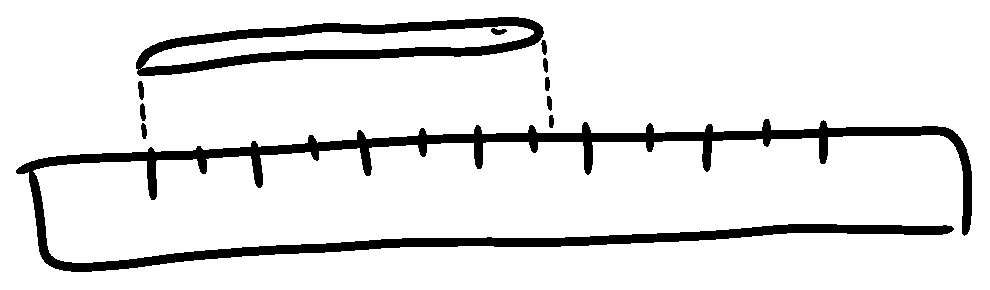
\includegraphics[width=0.6\linewidth]{images/Length}
    
    \caption{
      Рациональные числа~---~когда для измерения чего-то натуральных уже не хватает.
      (Но ``идеальную точность'' достигнуть нельзя~---~довольствуемся приближениями.)
    }
    \label{fig:rationals}
  \end{figure}
  
  \begin{figure}[ht]
    \centering
    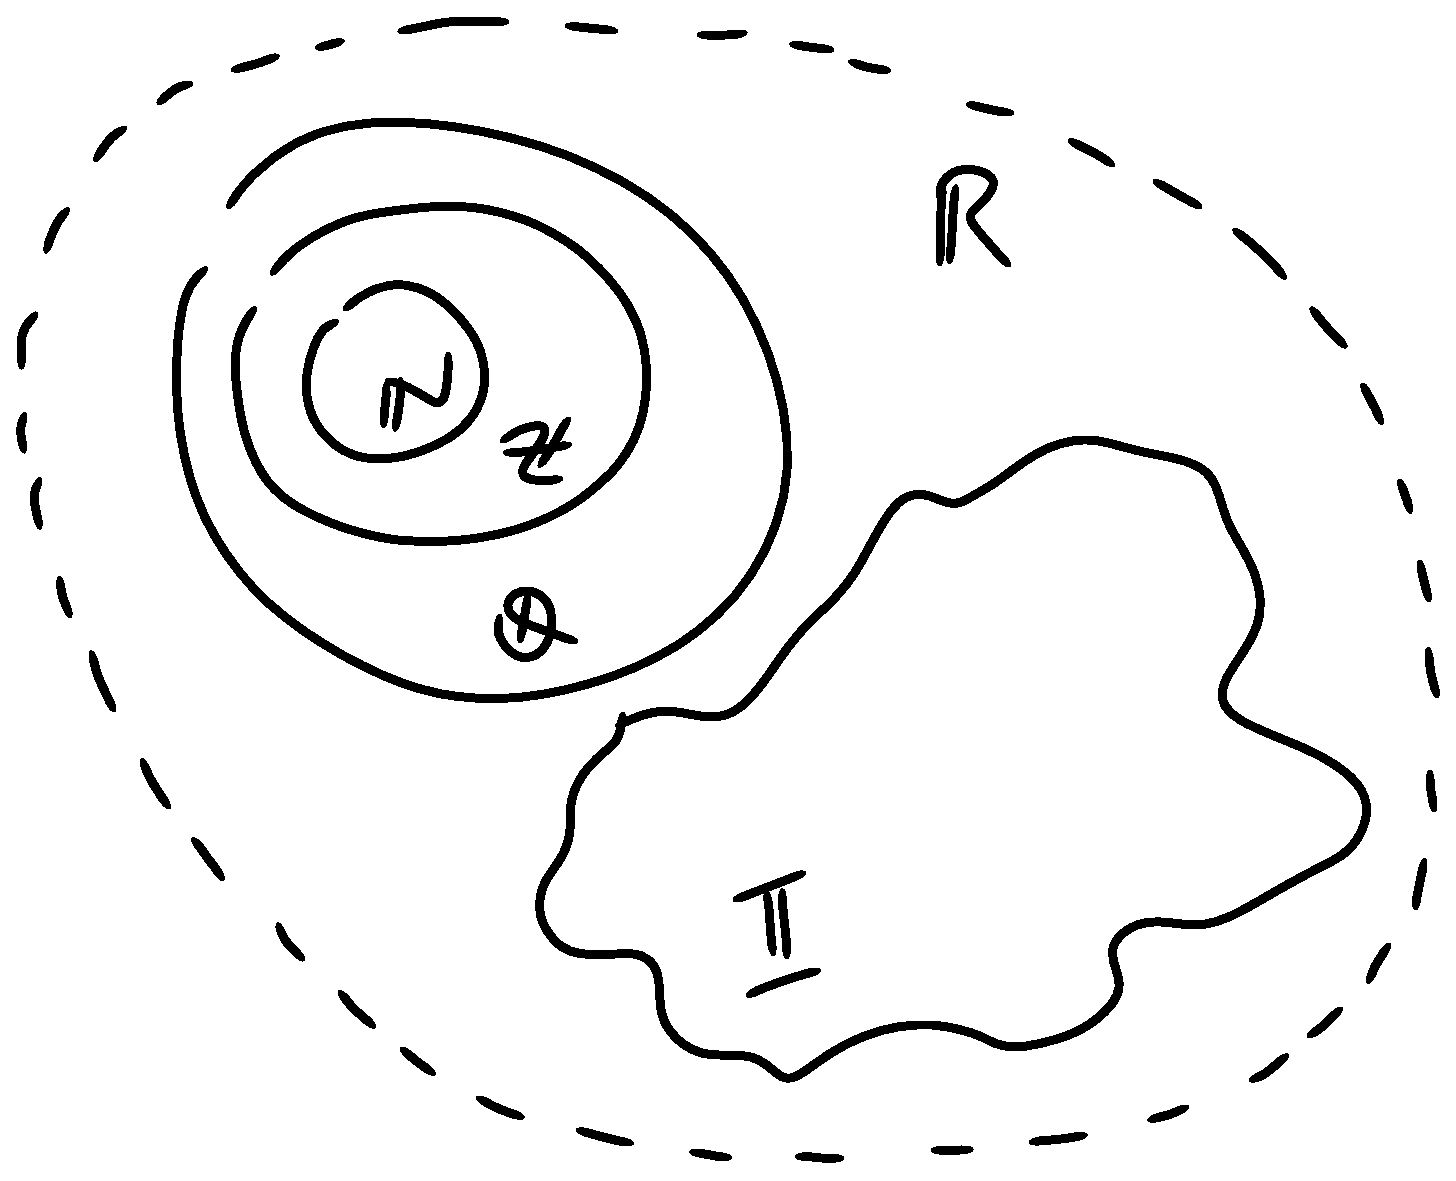
\includegraphics[width=0.6\linewidth]{images/Numbers}
    
    \caption{
      Иррациональные числа~---~``не такие, как рациональные'' (всё, что не попадает чётко на штрихи, отмеченные на линейке).
    }
    \label{fig:irrationals}
  \end{figure}
  
  Кроме этого, выделяют ещё \emph{ноль} и \emph{отрицательные числа}.
  Вводится множество \emph{целых} чисел~---~натуральные числа, противоположные им, и ноль.
  А рациональные и иррациональные могут быть как больше, так и меньше нуля.
  ``Вообще все-все'' числа (рациональные и иррациональные) образуют множество \emph{действительных} чисел.
  
  Более формально, действительное число~---~такое, которое может быть представлено в виде десятичной дроби (конечной или бесконечной).
  Рациональное число~---~это такое, которое может быть представлено в виде $\frac{p}{q}$, где $p \hm\in \ZZ$, а $q \hm\in \NN$.
  При этом также верно, что \emph{рациональные числа и только они представимы в виде конечных или бесконечных периодических десятичных дробей}.
  
  \begin{example}
    Периодическая десятичная дробь~---~такая, у которой дробная часть с какого-то момента строится бесконечным повторением какого-то фрагмента.
    Например:
    \[
      1{,}0809202420242024\ldots \hm= 1{,}0809(2024)
    \]
    
    Получим представление приведённого числа в виде обычной дроби.
    Для этого надо как-то ``избавиться'' от бесконечной части.
    И можно прийти к такому способу:
    \[
      \begin{aligned}
        &10000 \cdot 1{,}0809(2024) = 10809{,}2024(2024)\\
        &10000 \cdot 1{,}0809(2024) - 1{,}0809(2024) = 10809{,}2024 - 1{,}0809
      \end{aligned}
    \]
    
    И в итоге в виде дроби число выражается так:
    \[
      1{,}0809(2024) = \frac{10809{,}2024 - 1{,}0809}{10000 - 1} = \frac{108092024 - 10809}{9999 \cdot 10000}
    \]
  \end{example}
  
  % TODO: пример про девятку в периоде
  
  Кроме самих чисел (``придуманных объектов'') существуют ещё действия, которые можно с ними делать (``придуманные операции'').
  Например, сложение.
  Со сложением натуральных чисел ``всё понятно'': $1 \hm+ 1 \hm= 2$.
  Однако при сложении рациональных уже приходится пользоваться ``правилами'', как вообще их складывать.
  (А как сложить два иррациональных числа?..)
  Но даже с натуральными числами может быть не так просто: если за ``абстрактными'' числами стоят какие-то реальные объекты, а за ``абстрактным'' сложением~---~какое-то ``реальное'', работающее по своим правилам.
  Например, ``одна счётная палочка'' + ``ещё одна палочка'' = ``две палочки''.
  Но ``масса одного нуклона'' + ``масса другого нуклона'' > ``массы ядра, состоящего из этих нуклонов''.
  Или распродажное ``1 + 1 = 3'' (``купи две перчатки~---~получи третью в подарок'').
  
  В общем, на числа, как и на операции с ними~---~можно смотреть как отчасти на придуманные ``правила игры'', как на модель (возможно) чего-то ``реального'', живущего по своим (возможно, не до конца известным) правилам...
  
  % TODO: только условие плюс строчка решения уместились внизу страницы
  \newpage
  
  
  \subsection{С1, \S 3, \textnumero 4}
  
  Доказать, что для любых рациональных чисел $a$ и $b$, таких что $a \hm< b$, найдётся иррациональное число $c$, удовлетворяющее условию $a \hm< c \hm< b$.%\footnote{Можно ли оценить вероятность ...} % TODO
  
  \begin{solution}
  
    \mbox{}\par
    \emph{Вариант 1, где проводится сопоставление с отрезком, для которого точно ``всё хорошо''}.
    
    Известно, что $\sqrt 3 \hm\in \II$.\footnote{
      От противного: допустим, $\sqrt 3 \hm\in \QQ$.
      Тогда $\sqrt 3 \hm= \frac{p}{q}$, где $p \hm\in \ZZ$, $q \hm\in \NN$.
      Домножая на $q$ обе части равенства и потом ещё возводя в квадрат, получаем: $3 q^2 \hm= p^2$.
      Но такого не может быть, потому что если разложить на простые множители левую и правую части, то слева множитель $3$ будет в нечётной степени, а справа~---~в чётной.
      Противоречие.
      Значит, $\sqrt 3 \hm\in \II$.
    }
    При этом $\sqrt 3 \hm\approx 1{,}7{\ldots} \in [1, 2]$.
    То есть на отрезке $[1, 2]$ точно есть хотя бы одно иррациональное число.
    
    Вернёмся теперь к ``абстрактному'' отрезку $[a, b]$ из условия.
    Можно заметить, что каждое число этого отрезка можно представить в виде ``$a$ плюс сдвиг''.
    Так, $a \hm= a \hm+ 0$, $b \hm= a \hm+ (b \hm- a)$~---~а у всех внутренних точек сдвиг варьируется от $0$ до $(b \hm- a)$:
    \begin{equation}
    \begin{split}
      x \in [a, b] &\leftrightarrow x = a + s,\ s \in [0, b - a]\\
                   &\leftrightarrow x = a + d (b - a),\ d \in [0, 1]
    \end{split}
    \end{equation}
    где в последнем переходе сдвиг был выражен через параметр $d \hm\in [0, 1]$ как ``доля длины отрезка $[a, b]$''.\footnote{
      Символом $\leftrightarrow$ обозначена ``равносильность переходов'': если ``слева'', то и ``справа'' ($\rightarrow$), и если ``справа'', то и ``слева'' ($\leftarrow$).
    }
    
    Но точно такое же представление точек можно привести и для точек ``заведомо хорошего'' отрезка $[1, 2]$:
    \[
      x \in [1, 2] \leftrightarrow x = 1 + d (2 - 1) = 1 + d,\ d \in [0, 1]
    \]
    
    Получаем \emph{взаимно однозначное соответствие} между точками отрезков $[a, b]$ и $[1, 2]$: точки с одинаковыми значениями~$d$ ``связаны'' (если на отрезке $[a, b]$ точке $x_0$ соотвествует сдвиг с параметром $d_0$, то на отрезке $[1, 2]$ найдётся единственная точка $y_0$, которой соответствует сдвиг с таким же $d_0$, и наоборот).
    Посмотрим, какая точка $x^*$ отрезка $[a, b]$ соответствует точке $\sqrt 3 \hm\in [1, 2]$.
    Пусть $\sqrt 3 \hm= 1 \hm+ d^*$.
    Тогда и $x^* \hm= a \hm+ d^* (b - a)$.
    Но из представления $\sqrt 3$ как суммы $1 \hm+ d^*$ следует, что доля $d^* \hm\in \II$!
    А потому и $x^* \hm\in \II$.
    
    \medskip
    
    \emph{Вариант 2, где просто находится нужное $c$}.
    
    В прошлом сюжете рассматривались сдвиги от начальной точки отрезка.
    А можно ли из $a$ просто сразу ``перепрыгнуть'' в иррациональное число?
    Да, можно, если величина ``прыжка'' будет иррациональной и не очень большой (чтоб не вылететь на пределы $[a, b]$).
    Приведём пример такого ``прыжка'':
    \[
      x^* = a + \frac{\sqrt{3}}{100} (b - a)
    \]
    
    \emph{Вариант 3, где $c$ не находится в явном виде, но немного ``замороченно'' строится руками}.
    
    Перепрыгнуть сразу в иррациональное число~---~можно, но, возможно, не очень интересно.
    Поэтому теперь последовательно построим руками ``своё'' иррациональное число!
    
    Пусть, для наглядности, $a \hm= 1{,}729$ и $b \hm= 1{,}730$.
    Начнём строить иррациональное число из отрезка $[a, b]$.
    В первом ``приближении'' возьмём $x_1 \hm= 1{,}729$ (то есть просто $x_1 \hm= a$).
    Далее, уйдём чуть в сторону от $a$ (за $b$ уже точно не перелетим): $x_2 \hm= 1{,}7291$.
    Оба $x_1$ и $x_2$ рациональные...
    И как бы мы ни ``плодили'' ещё цифр справа после запятой~---~всё равно десятичная дробь будет конечной.
    Иррациональное же число не представимо ни в виде конечной, ни в виде бесконечной периодической десятичной дроби.
    Поэтому надо предложить алгоритм, такой чтоб \emph{в пределе} (при неограниченном количестве присоединений ещё одной цифры справа) получалась бесконечная непериодическая дробь.
    Сделать так, чтоб дробь была просто бесконечной~---~не сложно.
    Можно, например, просто бесконечное число раз приписывать справа единицу:
    \[
      \begin{aligned}
        &x_1 = 1{,}729\\
        &x_2 = 1{,}7291\\
        &x_3 = 1{,}72911\\
        &\ldots\\
        &x_n = 1{,}72911 \ldots 1\\
        &\ldots
      \end{aligned}
    \]
    Но в таком случае, очевидно, в пределе получаем $1{,}729(1)$~---~периодическая десятичная дробь, а потому число рациональное.
    Нужно как-то ``предотвратить'' образование периода в дроби...
    Поэтому опять будем приписывать справа единицы, но, например, будем чередовать их с двойками, так чтобы периода никогда не возникло:
    \[
      \begin{aligned}
        &x_1 = 1{,}729\\
        &x_2 = 1{,}7291\\
        &x_3 = 1{,}72912\\
        &x_4 = 1{,}729121\\
        &x_5 = 1{,}7291212\\
        &x_6 = 1{,}72912122\\
        &x_7 = 1{,}729121221\\
        &\ldots\\
        &x_n = 1{,}729121221222122221222221\ldots
      \end{aligned}
    \]
    Число $x^*$, получаемое в пределе при $n \hm\to +\infty$ (при переходе в члену последовательности $x_n$ со всё более высоким номером, то есть при бесконечном дописывании справа цифр по описанному выше алгоритму), лежит на отрезке $[a, b]$ и по построению является бесконечной непериодической десятичной дробью, а потому иррациональное.
    (Видно, что по такой ``схеме'' можно построить ещё сколько угодно иррациональных чисел на заданном отрезке.)
  \end{solution}
  
  
  
  
  \section{Производная}
  
  % TODO: copy-paste раздела про функции из Geome

  % https://ru.wikipedia.org/wiki/%D0%9F%D1%80%D0%BE%D0%B8%D0%B7%D0%B2%D0%BE%D0%B4%D0%BD%D0%B0%D1%8F_%D1%84%D1%83%D0%BD%D0%BA%D1%86%D0%B8%D0%B8  
  % https://ru.wikipedia.org/wiki/%D0%9F%D1%80%D0%BE%D0%B8%D0%B7%D0%B2%D0%BE%D0%B4%D0%BD%D0%B0%D1%8F_%D1%84%D1%83%D0%BD%D0%BA%D1%86%D0%B8%D0%B8#/media/%D0%A4%D0%B0%D0%B9%D0%BB:Derivative_of_a_function.svg
  \begin{figure}[ht]
    \centering
    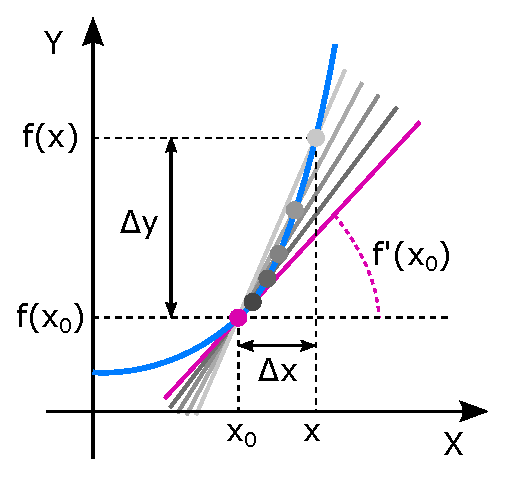
\includegraphics[width=0.8\linewidth]{images/Derivative_of_a_function}
    
    \caption{
      Производная функции~$f(x)$ в точке~$x_0$~---~тангенс угла наклона касательной к графику функции в этой точке.
      А касательная~---~как \emph{предел} секущей при приближении второго её конца в $x_0 \hm+ \Dt x$ к интересуемой точке: $\Dt x \hm\to 0$.
      (Таким образом, чтобы можно было говорить о производной функции в точке, функция должна быть определена как в самой точке, так и рядом с ней~---~в её \emph{окрестности}.)
      (Источник картинки: \href{https://commons.wikimedia.org/wiki/File:Derivative\_of\_a\_function.svg}{commons.wikimedia.org/wiki/File:Derivative\_of\_a\_function.svg}.)
    }
    \label{fig:derivative}
  \end{figure}
  
  Пусть есть функция $f\hm\colon X \hm\to \RR$, $X \hm\subseteq \RR$.
  Пусть $x_0 \hm\in X$, и функция определена в некоторой окрестности точки $x_0$\footnote{Иными словами, $x_0$~---~\emph{внутренняя точка} $X$.} (определена во всех точках ``рядом'' с $x_0$).
  Тогда производной функции $f(x)$ в точке~$x_0$ называется следующий предел (если он существует):
  \[
    f'(x_0) = \lim_{x \to x_0} \frac{f(x) - f(x_0)}{x - x_0}
  \]
  
  Или, в немного других обозначениях:
  \[
    f'(x_0) = \lim_{\Dt x \to 0} \frac{f(x_0 + \Dt x) - f(x_0)}{\Dt x}
  \]
  
  Саму производную тоже есть несколько вариантов, как обозначать.
  Так,
  \[
    f'(x_0) \equiv f'(x)|_{x = x_0}
  \]
  (запись справа~---~подстановка, её смысл: ``взяли производную, получили функцию $f'(x)$, и потом подставили вместо $x$ конкретную точку $x_0$, в которой хотим узнать значение производной'').
  Или, ещё способ:
  \[
    f'(x_0) = \frac{\diff f(x_0)}{\diff x}
  \]
  где $\diff$ означает \emph{дифференциал}.\footnote{
    О дифференциале ``с физической точки зрения'' часто думают как о ``(бесконечно) малом приращении''.
    Но на математике так лучше не говорить, потому что такому определению ``недостаёт точности'' (хотя бы потому, что не понятно, насколько всё-таки малое). % TODO: smeat smile
    С другой стороны, что-то про ``малость дифференциала'' есть и в математике...
    Дифференциал функции в точке~---~это просто линейная функция от дифференциала аргумента: $\diff f(x_0) \hm\equiv f'(x_0) \diff x$ (функция, проходящая через точку $x_0$ с наклоном $f'(x_0)$).
    Дифференциал аргумента~---~это просто приращение аргумента: $\diff x \hm= x \hm- x_0$.
    Но при приближении к $x_0$ приращение функции становится всё больше ``похоже'' на дифференциал, так что в пределе отношение ``малых приращений'' в самом деле становится равно отношению дифференциалов, то есть производной (``касательная в пределе становится секущей'').
  }
  Отсюда же можно получить выражение для дифференциала функции в точке:
  \[
    \diff f(x_0) = f'(x_0) \diff x
  \]
  
  \begin{example}
    Найдём из определения производную функции $f(x) \hm= x^2$, $x \hm\in \RR$.
    
    Пусть $x_0 \hm\in \RR$.
    Тогда производная в этой точке:
    \begin{equation*}
    \begin{split}
      f'(x_0) = \lim_{\Dt x \to 0} \frac{f(x_0 + \Dt x) - f(x_0)}{\Dt x}
        &= \lim_{\Dt x \to 0} \frac{(x_0 + \Dt x)^2 - x_0^2}{\Dt x}\\
        &= \lim_{\Dt x \to 0} \frac{2 x_0 \Dt x + \Dt^2 x}{\Dt x}
        = \lim_{\Dt x \to 0} (2 x_0 + \Dt x)
        = 2 x_0
    \end{split}
    \end{equation*}
    (где в последнем переходе при вычислении предела уже ничего не мешало ``просто занулить'' $\Dt x$).
    
    Таким образом, $f'(x) \hm= 2x$.
  \end{example}
  
  
  \subsection{Некоторые свойства производной}
  
  Из определения производной следует, что производная обладает свойством \emph{линейности}:
  \[
    \begin{aligned}
      &\bigl(\alpha f(x)\bigr)' = \alpha f'(x),\quad \alpha \in \RR\\
      &\bigl(f(x) + g(x)\bigr)' = f'(x) + g'(x)
    \end{aligned}
  \]
  
  Производная произведения функций $(fg)(x) \hm= f(x) g(x)$:
  \begin{equation}
    \boxed{(fg)' = f' g + f g'}
  \end{equation}
  
  Проверим:
  \[
    (fg)'(x_0) = \lim_{\Dt x \to 0} \frac{f(x_0 + \Dt) g(x_0 + \Dt) - f(x_0) g(x_0)}{\Dt x} = \blacktriangle
  \]
  
  Добавим и вычтем в числителе \textcolor{pink}{слагаемое}, так чтобы можно было перегруппировать, вынести за скобку общий множитель и прийти к разности значений в точках ``одиночных'' функций $f$ и $g$:
  \begin{equation}\label{eq:d-prod}
  \begin{split}
    \blacktriangle &= \lim_{\Dt x \to 0} \frac{\bigl(f(x_0 + \Dt x) g(x_0 + \Dt x) - \textcolor{pink}{f(x_0) g(x_0 + \Dt x)}\bigr) + \bigl(\textcolor{pink}{f(x_0) g(x_0 + \Dt x)} - f(x_0) g(x_0)\bigr)}{\Dt x}\\
      &= \lim_{\Dt x \to 0} \frac{\bigl(f(x_0 + \Dt x) - f(x_0)\bigr) g(x_0 + \Dt x) + f(x_0) \bigl(g(x_0 + \Dt x) - g(x_0)\bigr)}{\Dt x}\\
      &= \lim_{\Dt x \to 0} \frac{\bigl(f(x_0 + \Dt x) - f(x_0)\bigr) g(x_0 + \Dt x)}{\Dt x} + \lim_{\Dt x \to 0} \frac{f(x_0) \bigl(g(x_0 + \Dt x) - g(x_0)\bigr)}{\Dt x}\\
      &= f'(x_0) g(x_0) + f(x_0) g'(x_0)
  \end{split}
  \end{equation}
  
  Производная частного функций $\frac{f(x)}{g(x)}$:
  \begin{equation}
    \boxed{\left(\frac{f}{g}\right)' = \frac{f'g - fg'}{g^2}}
  \end{equation}
  
  Показать это можно, сведя всё к уже рассмотренному ранее произведению:
  \[
    \left(\frac{f}{g}\right)' = \left(fg^{-1}\right)'
      = f'g^{-1} + f \left(g^{-1}\right)'
      = \frac{f'}{g} + f \cdot \left(y^{-1}\right)'|_{y = g} \cdot g'
      = \frac{f'}{g} - f \cdot \frac{1}{g^2} \cdot g'
      = \frac{f'g - fg'}{g^2}
  \]
  
  
  \subsection{Производная сложной функции}
  
  \begin{figure}[ht]
    \centering
    \includegraphics[width=0.6\linewidth]{images/X-Y-Z}
    
    \caption{
      Функции $f\colon X \hm\to Y$ и $g\colon Y \hm\to Z$ и сложная функция $\phi\colon X \hm\to Z$, $\phi(x) = g\bigl(f(x)\bigr)$.
    }
    \label{fig:x-y-z}
  \end{figure}
  
  Пусть есть функции $f\colon X \hm\to Y$ и $g\colon Y \hm\to Z$.
  Пусть $x_0 \hm\in X$, $f(x_0) \hm\equiv y_0$.
  Тогда если существуют производные $f'(x_0)$ и $g'(y_0)$, то производная \emph{сложной функции} $\phi(x) = g\bigl(f(x)\bigr)$~(см. рисунок~\ref{fig:x-y-z}) равна:
  \begin{equation}
    \phi'(x_0) = \left.\Bigl(g\bigl(f(x)\bigr)\Bigr)'\right|_{x = x_0} = g'(y_0)|_{y_0 = f(x_0)} f'(x_0)
  \end{equation}
  
  Это тоже можно показать из определения производной (с парой ``махинаций'' типа ``добавления/убирания'' \textcolor{pink}{чего-то}~\eqref{eq:d-prod}):
  \begin{equation*}
  \begin{split}
    \phi'(x_0) &= \lim_{\Dt x \to 0} \frac{g\bigl(f(x_0 + \Dt x)\bigr) - g\bigl(f(x)\bigr)}{\Dt x}\\
      &= \lim_{\Dt x \to 0} \frac{g\bigl(f(x_0 + \Dt x)\bigr) - g\bigl(f(x)\bigr)}{\textcolor{pink}{f(x_0 + \Dt x) - f(x_0)}} \cdot \frac{\textcolor{pink}{f(x_0 + \Dt x) - f(x_0)}}{\Dt x}\\
      &= \lim_{\Dt y \to 0} \frac{g(y_0 + \Dt y) - g(y_0)}{y - y_0} \cdot \lim_{\Dt x \to 0} \frac{f(x_0 + \Dt x) - f(x_0)}{\Dt x}\\
      &= g'(y_0) f'(x_0)
  \end{split}
  \end{equation*}
  
  
  \subsection{Некоторые табличные производные}
  
  Приведём ``базовые'' производные.
  
  \begin{equation}
    (x^{\alpha})' = \alpha x^{\alpha - 1},\quad \alpha \in \RR,\ x > 0\quad (\mbox{или}\ \alpha \in \NN,\ x \in \RR)
    % TODO: письмо про это (https://en.wikipedia.org/wiki/Exponentiation#Powers_via_logarithms)
  \end{equation}
  
  \begin{equation}
    (e^x)' = e^x
  \end{equation}
  
  \begin{equation}
    (a^x)' = a^x \ln a
  \end{equation}
  
  \begin{example}
    Покажем последнюю формулу:
    \[
      (a^x)' = \left(e^{x \ln a}\right)' = \left(e^{y}\right)'|_{y = x \ln a} \cdot (x \ln a)' = a^x \cdot \ln a
    \]
  \end{example}
  
  \begin{equation}
    \ln' x = \frac{1}{x}
  \end{equation}
  
  \begin{equation}
    \sin'{x} = \cos{x}
  \end{equation}
  
  \begin{equation}
    \cos'{x} = {-}\sin{x}
  \end{equation}
  
  \begin{equation}
    \tg'{x} = \frac{1}{\cos^2{x}}
  \end{equation}
  
  \begin{equation}\label{eq:d-arcsin}
    \arcsin'{x} = \frac{1}{\sqrt{1 - x^2}}
  \end{equation}
  
  \begin{example}
    Посмотрим, почему получается такое выражение для производной арксинуса.
    Область значений $\arcsin$ есть $\left[{-}\frac{\pi}{2}, \frac{\pi}{2}\right]$.
    Значит, на этом промежутке $\arcsin$ будет функцией, \emph{обратной} функции $\sin$:
    \[
      \arcsin \sin x = x,\quad x \in \left[{-}\frac{\pi}{2}, \frac{\pi}{2}\right]
    \]
    
    С другой стороны, $\sin$ будет обратной для $\arcsin$ (на другом промежутке):
    \[
      \sin \arcsin x = x,\quad x \in [-1, 1]
    \]
    
    Продифференцируем последнее равенство:
    \[
      \begin{aligned}
        &(\sin \arcsin x)' = x'\\
        &\sin' y|_{y = \arcsin x} \cdot \arcsin' x = 1\\
        &\cos \arcsin x \cdot \arcsin' x = 1
      \end{aligned}
    \]
    
    Откуда получаем:
    \[
      \arcsin' x = \frac{1}{\cos \arcsin x}
    \]
    
    % TODO: картинка с окружностью
    Но так как $\arcsin x \hm\in \left[{-}\frac{\pi}{2}, \frac{\pi}{2}\right]$, то $\cos \arcsin x \hm> 0$.
    Поэтому можно выразить косинус следующим образом (корень с ``плюсом''):
    \[
      \cos \arcsin x = \sqrt{1 - \sin^2 \arcsin x} = \sqrt{1 - x^2}
    \]
    
    В результате имеем~\eqref{eq:d-arcsin}.
  \end{example}
  
  \begin{equation}
    \arctg' x = \frac{1}{1 + x^2}
  \end{equation}
  
  \begin{example}
    % TODO: картинка
    Найдём производную функции $y \hm= |x|$.
    
    Если нарисовать график функции, то будет видно, что в любой его точке, кроме $x \hm= 0$, можно провести единственную касательную: правее нуля тангенс угла наклона будет равен $+1$, левее он будет $-1$.
    В нуле же можно провести несколько касательных, поэтому производная в этой точке не определена.
    
    Если решать не графически, а аналитически, то можно просто раскрыть модуль и рассмотреть функцию на двух участках:
    \[
      y = \left\{
        \begin{aligned}
          &\hphantom{{+}}x,\quad x \geq 0\\
          &{-}x,\quad x < 0
        \end{aligned}
      \right.
    \]
    
    Тогда производная:
    \[
      y' = \left\{
        \begin{aligned}
          &\hphantom{{+}}1,\quad x > 0\\
          &{-}1,\quad x < 0
        \end{aligned}
      \right.
    \]
    
    При взятии производной из первого условия $x \hm\geq 0$ был исключён ноль, потому что это ``крайняя'' точка промежутка~---~а чтобы производная существовала, функция должна быть определена в окрестности (то есть таким образом, разбивкой на случаи ``$x \hm\geq 0$''/``$x \hm< 0$'' производную в нуле не найти).
    Точку ноль можно бы было рассмотреть отдельно, попытавшись найти производную в ней по определению.
    Но это бы тоже ни к чему не привело, потому что при ``движении'' в разные стороны от нуля (влево или вправо, то есть $\Dt x \hm< 0$ или $\Dt x \hm> 0$) получались бы разные производные, чего быть не может.
  \end{example}
  
  
  \subsection{С1, \S 13, \textnumero 32}
  
  Найти производную функции $y \hm= f(x)$ и указать её область существования: % или ``область её существования''?
  \[
    y = \log_x 2^x
  \]
  
  \begin{solution}
    Логарифм с переменным основанием~---~такой функции нет среди ``табличных производных''.
    Но можно перейти к новому основанию (фиксированному):
    \begin{equation}\label{eq:1-13-32}
      \log_x 2^x = \frac{\ln 2^x}{\ln x}
    \end{equation}
    
    Теперь можно воспользоваться правилом вычисления производной частного:
    \[
      \left(\frac{\ln 2^x}{\ln x}\right)' = \frac{(\ln 2^x)' \ln x - \ln 2^x (\ln x)'}{\ln^2 x} = \blacktriangle
    \]
    
    Производная сложной функции в числителе:\footnote{
      Или, если предварительно упростить, можно было обойтись и без сложной функции: $\ln 2^x \hm= x \ln 2 \Rightarrow (\ln 2^x)' \hm= (x \ln 2)' = \ln 2$.
    }\textsuperscript{,}\footnote{
      (И упрощать тогда уж лучше было ещё раньше, выражение~\eqref{eq:1-13-32} для самой функции~$f(x)$...)
    }  % https://tex.stackexchange.com/questions/28465/multiple-footnotes-at-one-point
    \[
      (\ln 2^x)' = \left.\frac{1}{y}\right|_{y = 2^x} \cdot (2^x)' = \frac{1}{2^x} \cdot 2^x \ln 2 = \ln 2
    \]
    
    Поэтому, возвращаясь к производной $f'(x)$:
    \[
      \blacktriangle = \frac{\ln 2 \ln x - \ln 2^x \frac{1}{x}}{\ln^2 x} = \frac{\ln 2 (\ln x - 1)}{\ln^2 x}
    \]
    
    Область определения $f'(x)$:
    \[
      \left\{
        \begin{aligned}
          &x > 0\\
          &\ln^2 x \not= 0
        \end{aligned}
      \right. \leftrightarrow
      \left\{
        \begin{aligned}
          &x > 0\\
          &x \not= 1
        \end{aligned}
      \right. \leftrightarrow x \in (0, 1) \cup (1, +\infty)
    \]
  \end{solution}
  
  
  \subsection{С1, \S 13, \textnumero 79}
  
  Найти производную функции $y \hm= f(x)$:
  \[
    y = \sin \ln |x|
  \]
  
  \begin{solution}
    Данная в условии функция является ``сложной-сложной'' функцией:
    \[
      y = \sin\Bigl( \ln\bigl( |x| \bigr) \Bigr)
    \]
    
    Поэтому её производная (две ступени ``разворачивания''):
    \begin{equation*}
    \begin{split}
      y' &= \sin'{z}|_{z = \ln |x|} \cdot \ln'{y}|_{y = |x|} \cdot |x|'\\
      &= \cos{z}|_{z = \ln |x|} \cdot \left.\frac{1}{y}\right|_{y = |x|} \cdot \left\{
        \begin{aligned}
          &\hphantom{{+}}1,\quad x > 0\\
          &{-}1,\quad x < 0
        \end{aligned}
      \right.\\  % TODO: align derivatives on the three levels of equation
      &= \cos \ln |x| \cdot \frac{1}{|x|} \cdot \left\{
        \begin{aligned}
          &\hphantom{{+}}1,\quad x > 0\\
          &{-}1,\quad x < 0
        \end{aligned}
      \right.
    \end{split}
    \end{equation*}
    
    Можно заметить, что ``ветвление'' для случаев $x \hm> 0$ и $x \hm< 0$ можно убрать, придя к такому выражению:
    \[
      y' = \frac{\cos \ln |x|}{x}
    \]
  \end{solution}
  
  
  % Пропустили на семинаре (было мало времени), да и сейчас не вижу смысла её решать :)
  %\subsection{С1, \S 13, \textnumero 106}
  %
  %\begin{solution}
  %\end{solution}
  
  
  
  
  \section{Неопределённый интеграл}
  
  \begin{figure}[ht]
    \centering
    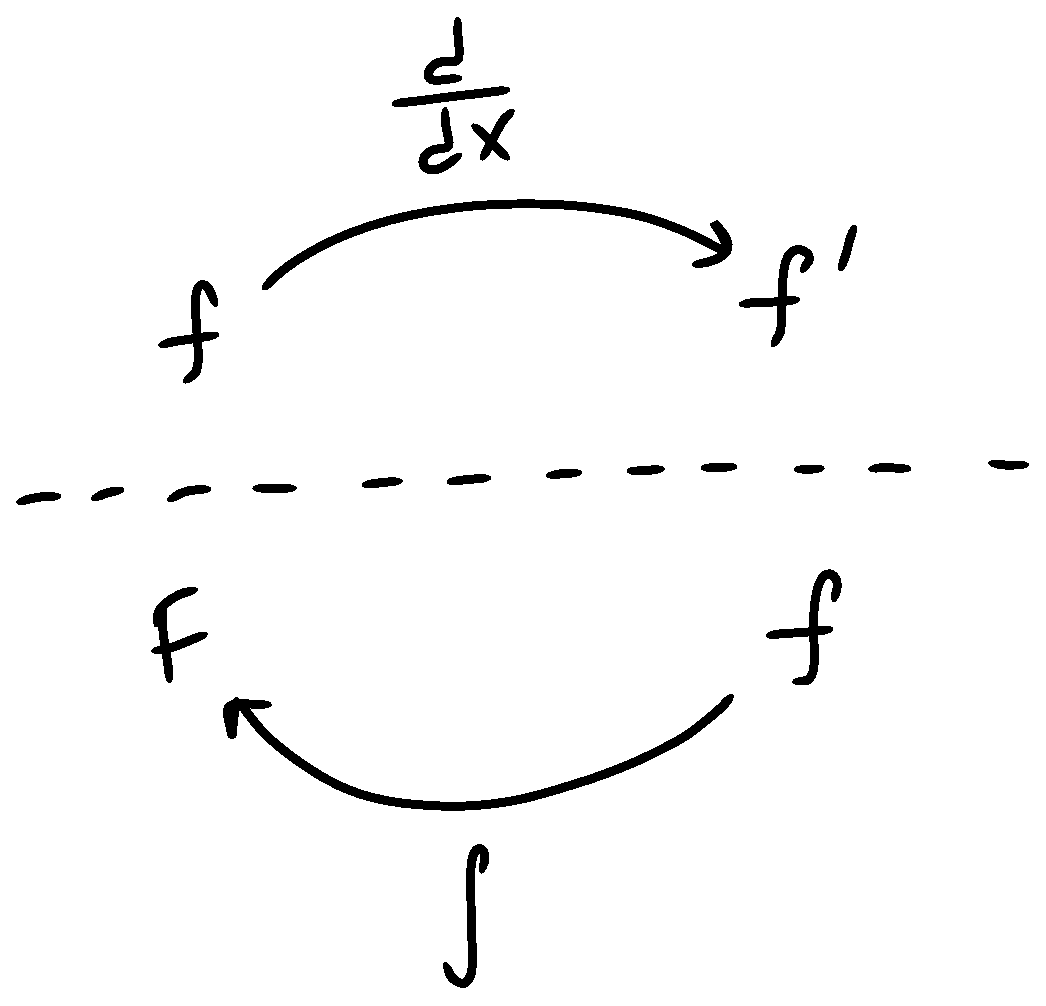
\includegraphics[width=0.5\linewidth]{images/Diff-Int}
    
    \caption{
      Об интегрировании можно думать как о действии, в некотором смысле обратном дифференцированию (в том смысле, что интегрирование действует ``в другую сторону'').
      Однако в строгом смысле интегрирование не является обратной операцией, хотя бы потому что результат взятия производной от функции~---~функция, результат же взятия неопределённого интеграла от функции~---~\emph{множество} функций.
    }  % TODO: в описании говорится о том, что ещё только будет введено
    \label{fig:diff-vs-int}
  \end{figure}
  
  \emph{Первообразной} функции $f(x)$ на некотором промежутке называется функция $F(x)$, такая что на данном промежутке $F'(x) \hm= f(x)$.
  
  \begin{example}
    Пусть $f(x) \hm= x$, $x \hm\in \RR$.
    Тогда $F(x) \hm= \frac{x^2}{2}$ будет первообразной.
    Но и $\frac{x^2}{2} \hm+ 1$ тоже будет первообразной, и $\frac{x^2}{2} \hm+ 10$, и вообще $F(x) \hm+ C$, $C \hm\in \RR$.
    
    Существуют ли первообразные ``другого'' вида?
    Пусть $F'(x) \hm= f(x)$ и $G'(x) \hm= f(x)$.
    Что можно сказать про связь между $F(x)$ и $G(x)$?
    \[
      F'(x) = G'(x) \leftrightarrow F'(x) - G'(x) = 0 \leftrightarrow \bigl(F(x) - G(x)\bigr)' = 0
    \]
    то есть производная функции $F \hm- G$ равна нулю на $\RR$ (промежуток, на котором $F(x)$ и $G(x)$ являются первообразными функции $f(x)$).
    Но в таком случае ``очевидно'', что это константная функция, то есть $F \hm- G \hm= C \hm\in \RR$.
    
    Поэтому все первообразные функции $f(x)$ имеют вид $F(x) \hm+ C$, $C \hm\in \RR$.
  \end{example}
  
  \emph{Неопределённым интегралом} функции $f(x)$ называется \emph{совокупность всех первообразных} этой функции~(см. рисунок \ref{fig:diff-vs-int}):
  \[
    \int f(x) \diff x = \{F(x) + C \mid C \in \RR\}
  \]
  где $F(x)$~---~какая-то одна первообразная.
  Обычно эту запись упрощают, опуская скобки, означающее множество (хотя это всё так же остаётся множеством):\footnote{
    В некоторых таблицах интегралов можно увидеть, что в упрощениях идут ещё дальше и пишут просто $\int f(x) \diff x \hm= F(x)$.
    Но на контрольных или экзаменах так точно писать не надо :)
  }
  \[
    \int f(x) \diff x = F(x) + C,\quad C \in \RR
  \]
  
  
  \subsection{Некоторые свойства неопределённого интеграла}
  
  Из определения производной и связи интеграла с производной:
  \[
    \int f'(x) \diff x = \int \diff f(x) = f(x) + C
  \]
  
  Из свойств производных следует свойство \emph{линейности} неопределённого интеграла:
  \[
    \left.
      \begin{aligned}
        &\int \alpha f(x) \diff x = \alpha \int f(x) \diff x,\quad \alpha \in \RR\\
        &\int \bigl(f(x) + g(x)\bigr) \diff x = \int f(x) \diff x + \int g(x) \diff x
      \end{aligned}
    \right.
  \]
  
  
  \subsection{Интегрирование по частям}
  
  Если существует интеграл вида $\int u(x) v'(x) \diff x$, то его можно считать следующим образом (формула интегрирования по частям):
  \begin{equation}\label{eq:by-parts}
    \int u v' \diff x = u v - \int v u' \diff x
  \end{equation}
  
  Формулу можно представить и в таком виде:
  \begin{equation}
    \int u \diff v = u v - \int v \diff u
  \end{equation}
  
  Убедимся, что~\eqref{eq:by-parts} ``работает''.
  В левой и правой частях формулы стоят множества первообразных.
  Пусть $F(x)$~---~какая-то первообразная у интеграла слева, то есть $F'(x) \hm= u v'$.
  Пусть $G(x)$~---~какая-то первообразная у интеграла справа, то есть $G'(x) \hm= vu'$.
  Но тогда в правой части формулы~\eqref{eq:by-parts} оказывается функция $uv \hm- G$, производная которой:
  \[
    (uv - G)' = (uv)' - G' = u'v + uv' - vu' = uv' = F'(x)
  \]
  совпадает с производной первообразной слева.
  Таким образом, первообразная слева лежит во множестве первообразных справа, и наоборот.
  То есть множества первообразных совпадают.
  О чём и говорит формула~\eqref{eq:by-parts}.
  
  
  \subsection{Некоторые табличные интегралы}
  
  Приведём формулы некоторых ``популярных'' интегралов.
  
  \begin{equation}
    \int x^\alpha \diff x = \frac{x^{\alpha + 1}}{\alpha + 1} + C,\quad \alpha \not= -1
  \end{equation}
  
  \begin{equation}\label{eq:int-to-ln}
    \int \frac{1}{x} \diff x = \ln |x| + C
  \end{equation}
  
  \begin{remark}
    Почему справа в~\eqref{eq:int-to-ln} стоит модуль?
    
    Если $x \hm> 0$, то очевидно, что $\ln' x \hm= \frac{1}{x}$.
    Однако подынтегральная функция $\frac{1}{x}$ определена и при $x \hm< 0$, поэтому и на этой области хорошо бы узнать первообразную.
    Убеждаемся, что
    \[
      \ln'{(-x)} = \left.\frac{1}{y}\right|_{y = -x} \cdot (-x)' = \frac{1}{-x} \cdot -1 = \frac{1}{x}
    \]
    
    Таким образом, в самом деле $\ln'{|x|} \hm= \frac{1}{x}$.
    (Ещё это можно попробовать представить графически.)
  \end{remark}
  
  % TODO: график функций
  
  \begin{equation}
    \int e^x \diff x = e^x + C
  \end{equation}
  
  \begin{equation}
    \int a^x \diff x = \frac{a^x}{\ln a} + C,\quad a > 0,\ a \not= 1
  \end{equation}
  
  \begin{example}
    Последнее соотношение можно проверить просто по производной, а можно и ``по-честному'' вычислить интеграл, сведя его к интегралу от~$e^x$.
    Сделаем это ради дополнительной демонстрации ``приёмов интегрирования'':
    \begin{equation*}
    \begin{split}
      \int a^x \diff x = \int e^{x \ln a} \diff x &= \frac{1}{\ln a} \int e^{x \ln a} \diff (x \ln a)\\
        &= \frac{1}{\ln a} \left.\int e^{y} \diff y \right|_{y = x \ln a} = \left.\frac{1}{\ln a} e^{y}\right|_{y = x \ln a} + C
        = \frac{a^x}{\ln a} + C
    \end{split}
    \end{equation*}
  \end{example}
  
  \begin{equation}
    \int \sin x \diff x = {-}\cos x + C
  \end{equation}
  
  \begin{equation}
    \int \cos x \diff x = \sin x + C
  \end{equation}
  
  \begin{equation}
    \int \frac{1}{\cos^2 x} \diff x = \tg x + C
  \end{equation}
  
  \begin{equation}
    \int \frac{1}{\sqrt{1 - x^2}} \diff x = \arcsin x + C
  \end{equation}
  
  \begin{example}
    Рассмотрим ещё ``усложнённую версию'' последнего интеграла (при $a \hm> 0$):
    \begin{equation*}
    \begin{split}
      \int \frac{1}{\sqrt{a^2 - x^2}} \diff x
        = \int \frac{1}{a \sqrt{1 - \left(\frac{x}{a}\right)^2}} \diff x
        &= \int \frac{1}{\sqrt{1 - \left(\frac{x}{a}\right)^2}} \diff \left(\frac{x}{a}\right)\\
        &= \left.\int \frac{1}{\sqrt{1 - y^2}} \diff y \right|_{y = x/a}
        = \arcsin{\left(\frac{x}{a}\right)} + C
    \end{split}
    \end{equation*}
    
    Итого:  
    \begin{equation}\label{eq:int-a-arcsin}
      \int \frac{1}{\sqrt{a^2 - x^2}} \diff x = \arcsin{\left(\frac{x}{a}\right)} + C,\quad a > 0
    \end{equation}
  \end{example}
  
  \begin{equation}
    \int \frac{1}{1 + x^2} \diff x = \arctg x + C
  \end{equation}
  
  Опять, усложним и по аналогии с примером выше получим:
  \begin{equation}\label{eq:int-a-arctan}
    \int \frac{1}{a^2 + x^2} \diff x = \frac{1}{a} \arctg\left(\frac{x}{a}\right) + C,\quad a \not= 0
  \end{equation}
  
  \begin{example}
    Помимо того, чтоб ``усложнять'', можно что-то поменять.
    Так, сделаем разность вместо суммы в знаменателе подынтегральной функции~\eqref{eq:int-a-arctan}:
    \[
      \int \frac{1}{x^2 - a^2} \diff x = \int \frac{1}{(x - a) (x + a)} \diff x = \blacktriangle
    \]
    
    ``Заметим'', что дробь, стоящая под интегралом, представима как сумма дробей:
    \[
      \frac{1}{(x - a) (x + a)} = \left(\frac{1}{x - a} - \frac{1}{x + a}\right) \cdot \frac{1}{2a}
    \]
    
    Поэтому интеграл можно переписать как сумму интегралов:
    \[
      \blacktriangle = \frac{1}{2a} \left(\int \frac{1}{x - a} \diff x - \int \frac{1}{x + a} \diff x\right)
        = \frac{1}{2a} \ln \left| \frac{x - a}{x + a} \right| + C
    \]
    
    Итого (``высокий логарифм''):  
    \begin{equation}
      \int \frac{1}{x^2 - a^2} \diff x = \frac{1}{2a} \ln \left| \frac{x - a}{x + a} \right| + C,\quad a \not= 0
    \end{equation}
  \end{example}
  
  Изменение же знаков в знаменателе~\eqref{eq:int-a-arcsin} приводит к такому интегралу (``длинный логарифм''):
  \begin{equation}
    \int \frac{1}{\sqrt{x^2 \pm a^2}} \diff x = \ln \left|x + \sqrt{x^2 \pm a^2}\right| + C,\quad a \not= 0
  \end{equation}
  % TODO: proof?
  
  
  \subsection{С2, \S 1, \textnumero 13(7)}
  
  Найти интеграл:
  \[
    J = \int \frac{1}{\sqrt{e^x - 1}} \diff x
  \]
  
  \begin{solution}
    Сделаем замену, \sout{в надежде, что это поможет}, упростив вид подынтегральной функции:
    \[
      \begin{aligned}
        &e^x = y,\quad y > 0\\
        &x = \ln y\\
        &\diff x = \diff (\ln y) = \ln'\! y \diff y = \frac{1}{y} \diff y
      \end{aligned}
    \]
    
    В результате замены приходим к интегралу вида:
    \[
      J = \int \frac{1}{\sqrt{y - 1}} \cdot \frac{1}{y} \diff y = \int \frac{1}{y \sqrt{y - 1}} \diff y
    \]
    
    Интеграл всё ближе к какому-то табличному.
    Единственное, что теперь ``мешает''~---~это корень в знаменателе (точнее, что в знаменателе стоит произведение одночлена на корень).
    Устраним корень ещё одной заменой, \sout{в надежде, что это упрощение не приведёт к усложнению чего-то другого}:
    \[
      \begin{aligned}
        &\sqrt{y - 1} = z,\quad z \geq 0\\
        &y = z^2 + 1\\
        &\diff y = \diff (z^2 + 1) = (z^2 + 1)' \diff z = 2z \diff z
      \end{aligned}
    \]
    
    Интеграл после замены:
    \[
      J = \int \frac{1}{(z^2 + 1) z} \cdot 2z \diff z = 2 \int \frac{1}{z^2 + 1} \diff z
    \]
    
    А это табличный интеграл, поэтому теперь остаётся только выписать первообразную и ещё провести обратные замены:
    \begin{equation*}
    \begin{split}
      J &= 2 \arctg z + C\\
        &= 2 \arctg \sqrt{y - 1} + C\\
        &= 2 \arctg \sqrt{e^x - 1} + C
    \end{split}
    \end{equation*}
  \end{solution}
  
  
  \subsection{С2, \S 1, \textnumero 23(1)}
  
  Найти интеграл:
  \[
    J = \int \ln^2 x \diff x
  \]
  % https://tex.stackexchange.com/questions/314610/spacing-in-integrals-with-latex
  
  \begin{solution}
    % https://tex.stackexchange.com/questions/32160/new-line-after-paragraph
    \mbox{}\par
    \emph{Способ 1: замена + по частям}.
    
    Заменим \sout{неудобный} ``нетабличный'' логарифм:
    \[
      \begin{aligned}
        &\ln x = y,\quad y \in \RR\\
        &x = e^y\\
        &\diff x = \diff (e^y) = e^y \diff y
      \end{aligned}
    \]
    
    Интеграл после замены:
    \[
      J = \int y^2 e^y \diff y
    \]
    
    А теперь можно несколько раз проинтегрировать по частям, чтобы $y^2$ ушла.
    Первое ``по-частям'':
    \begin{equation}
    \begin{split}
      J = \int y^2 \diff e^y
        = y^2 e^y - \int e^y \diff (y^2)
        = y^2 e^y - 2 \int y e^y \diff y
        = \blacktriangle
    \end{split}
    \end{equation}
    
    Второе ``по-частям'':
    \begin{equation}
    \begin{split}
      \blacktriangle = y^2 e^y - 2 \int y \diff (e^y)
        = y^2 e^y - 2 \left(y e^y - \int e^y \diff y\right)
        = y^2 e^y - 2 (y e^y - e^y) + C
    \end{split}
    \end{equation}
    
    Заменяя обратно $y$ на $x$, получаем:
    \[
      J = x \ln^2 x - 2(x \ln x - x) + C
    \]
    
    
    \emph{Способ 2: сразу по частям}.
    
    Можно попробовать интегрировать сразу по частям, без замены.
    При этом в качестве ``$\diff v$'' выступает просто $\diff x$:
    \[
      J = \int \ln^2 x \diff x
        = x \ln^2 x - \int x \diff (\ln^2 x)
        = \bigstar 
    \]
    
    Найдём отдельно дифференциал:
    \[
      \diff (\ln^2 x) = \left(\ln^2 x\right)' \diff x = 2 y|_{y = \ln x} \cdot \ln' x \diff x = 2 \frac{\ln x}{x} \diff x
    \]
    
    Возвращаясь к интегралу и беря аналогично второй раз по частям:
    \begin{equation}
    \begin{split}
      \bigstar = x \ln^2 x - 2 \int \ln x \diff x
               &= x \ln^2 x - 2 \left(x \ln x - \int x \diff \ln x\right)\\
               &= x \ln^2 x - 2 \left(x \ln x - \int \diff x\right)
               = x \ln^2 x - 2 (x \ln x - x) + C
    \end{split}
    \end{equation}
    
  \end{solution}
  
  
  \subsection{С2, \S 1, \textnumero 24(3)}
  
  Найти интеграл:
  \[
    J = \int e^{ax} \sin{bx} \diff x,\quad a^2 + b^2 \not= 0
  \]
  
  \begin{solution}
    Выражение $a^2 \hm+ b^2 \hm{\not=} 0$ есть лишь ``математичный'' способ сказать, что хотя бы один из коэффициентов $a$ и $b$ точно не ноль.
    
    Что можно сделать с $J$?
    Точно можно посмотреть на него как на интеграл вида $\int u \diff v$ и попробовать взять его по частям.
    Причём в качестве ``$\diff v$'' можно выбрать и $e^{ax} \diff x$, и $\sin{bx} \diff x$.
    Только вот дифференцирование ``$u$'' в этом случае (которая будет либо $\sin{bx}$, либо $e^{ax}$ соответственно) ни к чему хорошему вроде бы не приведёт (она не пропадёт)...
    Но ``по частям'' прямо напрашивается, да и других вариантов особо нет, к тому же ``не знаешь, что делать~---~делай то, что можешь''.
    В общем, по частям.
    
    Пусть $u \hm= e^{ax}$ и $\diff v \hm= \sin{bx} \diff x$.
    Преобразуем выражение для $\diff v$, выделив дифференциал функции:
    \begin{equation}\label{eq:2-1-24(3)-sinbxdx}
      \sin{bx} \diff x
        = \sin{bx} \diff \left(\frac{bx}{b}\right)
        = \frac{1}{b} \sin{bx} \diff (bx)
        = \frac{1}{b} \sin y \diff y|_{y = bx}
        = \frac{1}{b} \diff (-\cos y)|_{y = bx}
        = -\frac{1}{b} \diff \cos{bx}
    \end{equation}
    
    Из выражения выше видно, что мы ``неявно предположили'', что $b \hm{\not=} 0$.
    Хотя, возможно, могло быть и так, что $b \hm= 0$, но $a \hm{\not=} 0$.
    Но примем всё-таки, что $b \hm{\not=} 0$, и если получим ответ для этого случая, то потом уже посмотрим, имеет ли смысл рассматривать отдельно вариант $b \hm= 0$.

    Возвращаемся к интегралу:
    \[
      J = -\frac{1}{b} \int e^{ax} \diff \cos{bx}
        = -\frac{1}{b} \left(e^{ax} \cos{bx} - \int \cos{bx} \diff e^{ax}\right)
    \]
    
    Дифференциал функции в получившемся после интегрирования по частям новом интеграле:
    \begin{equation}\label{eq:2-1-24(3)-deax}
      de^{ax} = \left(e^{ax}\right)' \diff x = \left(e^{y}\right)'|_{y = ax} \cdot (ax)' \diff x = a e^{ax} \diff x
    \end{equation}
    
    Итого, выражение для интеграла~$J$ после применения ``по частям'':
    \begin{equation}\label{eq:2-1-24(3)-J-final}
      J = -\frac{1}{b} \Biggl(e^{ax} \cos{bx} - a \underbrace{\int e^{ax} \cos{bx} \diff x}_{I}\Biggr)
    \end{equation}
    
    Ничего хорошего вроде бы не получилось (а как будто даже наоборот).
    Зато снова есть возможность проинтегрировать по частям~---~интеграл~$I$, возникший в правой части.
    Так как $e^{ax}$ только что вынесли из-под дифференциала~\eqref{eq:2-1-24(3)-deax}, то занесём теперь под дифференциал функцию~$\cos bx$ (иначе придём ровно к тому же, с чего начали).
    (Преобразования аналогичны~\eqref{eq:2-1-24(3)-sinbxdx}):
    \[
      \cos{bx} \diff x = \frac{1}{b} \cos{bx} \diff (bx) = \frac{1}{b} \diff \sin{bx}
    \]
    
    Теперь берём по частям интеграл~$I$:
    \[
      I = \frac{1}{b} \int e^{ax} \diff \sin{bx}
        = \frac{1}{b} \left(e^{ax} \sin{bx} - \int \sin{bx} \diff e^{ax}\right)
        \overset{\eqref{eq:2-1-24(3)-deax}}{=} \frac{1}{b} \left(e^{ax} \sin{bx} - a \int e^{ax} \sin{bx} \diff x\right)
    \]
    
    Внимательно вглядываясь в получившееся выражение, можно заметить, что справа опять появился интеграл~$J$!
    \begin{equation}\label{eq:2-1-24(3)-I-final}
      I = \frac{1}{b} \left(e^{ax} \sin{bx} - a J\right)
    \end{equation}
    
    Но интеграл~$I$ сам возник ранее при вычислении~$J$~\eqref{eq:2-1-24(3)-J-final}.
    Поэтому, если подставить в~\eqref{eq:2-1-24(3)-J-final} вместо~$I$ выражение~\eqref{eq:2-1-24(3)-I-final}, то придём к уравнению относительно~$J$!\footnote{Всё-таки не совсем ``уравнению'', потому что $J$~---~это множество.}
    \[
      J = -\frac{1}{b} \left(e^{ax} \cos{bx} - a \cdot \frac{1}{b} \left(e^{ax} \sin{bx} - a J\right)\right) 
    \]
    
    Раскрывая скобки, перенося туда-сюда слагаемые из одной части в другую, упрощая (и не забывая добавить ``$+\, C$'', чтоб получить множество первообразных), получаем:
    \[
      J = \frac{e^{ax} (a \sin{bx} - b \cos{bx})}{a^2 + b^2} + C
    \]
    
    Вспомним, что мы начали с допущения $b \hm{\not=} 0$.
    Но видно, что в финальном ответе разрешается случай и $b \hm= 0$.
    Единственное, что важно~---~это что $a^2 \hm+ b^2 \hm{\not=} 0$.
    Но это дано по условию.
    Таким образом, интеграл нашли.
    (Можно было бы в самом начале по-другому выбрать $u$ и $\diff v$~---~путь вычислений был бы немного другой, но ответ бы получился такой же.)
  \end{solution}
  
  
  % \section{Последовательности. Предел последовательности}
\end{document}
